%=====================================================================
\section{Embedding-Space Analyses: Details}
\label{app:analyses}
%=====================================================================

All analyses in this section use the saved factorizations of 38 concepts $\times$ 5 seeds on Gemma-2-2B-it: \ember{}'s matrix with row sparsity (\ember{}), the sharpened matrix with row sparsity (\cs{}), and the sharpened matrix with global sparsity (\cs{}+\gs{}).
Unless stated otherwise, the concept feature of a run is identified without the judge, as the feature whose words match the concept's lexicon most often.

\subsection{Where the Concept's Energy Lies}
\label{app:energy}
\paragraph{Matrices and fits}
Raw $E_{\vs}^{\top}$; raw with $\hat\mu_B$ projected out; centred at $\mu_B$; whitened only ($\gamma = 0$); and \cs{}. Row-sparse fits, 38 concepts $\times$ 5 seeds; the 570 fits for the three intermediate matrices are new. A run ``finds'' the concept when its best feature has at least 5 lexicon words among its first 20 source words; no LLM judge is used.

\paragraph{Frequency}
Over 6.2M tokens of English Wikipedia, concept-only tokens are rarer than neutral-only ones in \expnum{35 of 38} concepts (median \expnum{9.4} vs.\ \expnum{12.9} per million), but their norms are not smaller (raw energy \expnum{0.9\%} larger). Across the vocabulary, a token's projection on $\hat\mu_B$ falls monotonically with its frequency (Spearman \expnum{$-0.69$} within a concept), and rare tokens put a smaller share of their centred energy on the top background directions (\expnum{0.07} vs.\ \expnum{0.65} at the frequent end). The tokens a raw concept feature collects are the rarest in $\vs$ (median \expnum{2.5} vs.\ \expnum{23} per million).

\paragraph{Seeded feature and full fits}
The seeded single feature (Figure~\ref{fig:mechanism}b) ends with purity \expnum{0.24} in the raw matrix, \expnum{0.04} centred and \expnum{0.27} with $\hat\mu_B$ projected out; whitening makes it pure (\expnum{0.86}, keeping \expnum{41\%} of the lexicon tokens) but ordinary (\expnum{70th} percentile of feature values), and sharpening raises its value to the \expnum{91st} percentile at the same purity (\expnum{37 of 38} concepts).
In full fits, a lexicon concept feature is found in \expnum{56\%} of raw runs, \expnum{61\%} with $\hat\mu_B$ projected out, \expnum{59\%} centred, \expnum{49\%} whitened only and \expnum{69\%} with \cs{}; per concept, raw $\to$ \cs{} is \expnum{15} better and \expnum{3} worse ($p = \expnum{0.011}$), and whitened only $\to$ \cs{} \expnum{17} and \expnum{0}.
The raw fit's best lexicon feature usually ranks near the top by $\rho$ (median rank \expnum{2}, against \expnum{1} under \cs{}; $p = \expnum{0.92}$); Harry Potter's raw rank is seed-dependent (\expnum{12, 1, 28, 48, 1}), while \cs{} ranks it first in all five seeds.

\paragraph{Selection-free directions}
The concept-minus-neutral mean direction, the top generalized eigenvector of concept vs.\ neutral second moments, and the top direction of the lexicon tokens do not rise in energy rank with \cs{} (e.g., lexicon direction rank \expnum{2} raw, which reflects $\hat\mu_B$; \expnum{9} without $\hat\mu_B$; \expnum{16.5} with \cs{}). What sharpening changes is the energy of the lexicon direction relative to whitening alone (\expnum{3.1$\times$} vs.\ \expnum{11.4$\times$} an average direction) and the value of the concept's cluster (App.~\ref{app:cs}).

\subsection{Feature Geometry and Norms}
\label{app:geometry}
\paragraph{Setup}
570 saved fits (\ember{}, \cs{} with row sparsity, \cinder{}), directions sign-aligned and compared in four metrics: the fit's own space, the raw embedding space (sharpened directions mapped back), the sharpened space (raw directions mapped forward), and the raw space with $\hat\mu_B$ projected out of every direction. Semantic relatedness of two features is the cosine of a small sentence encoder (all-MiniLM-L6-v2) between their source-word lists, independent of Gemma; token frequencies come from 32.6M tokens of Wikipedia.

\paragraph{Orthogonality}
Mean $|\cos|$ between directions:

\begin{center}
\footnotesize
\setlength{\tabcolsep}{3pt}
\begin{tabular}{@{}lccc@{}}
\toprule
Metric & \ember{} & \cs{}+RS & \cinder{} \\
\midrule
Own fit space & \expnum{.164} & \expnum{.052} & \expnum{.051} \\
Raw embedding space & \expnum{.164} & \expnum{.291} & \expnum{.258} \\
Raw, $\hat\mu_B$ projected out & \expnum{.079} & \expnum{.086} & \expnum{.079} \\
\bottomrule
\end{tabular}
\end{center}

\noindent Mapping sharpened directions back multiplies them by $T^{-1} \propto \Sigma_B^{1/2}$, which re-inflates the dominant background direction; $\hat\mu_B$ has cosine \expnum{0.82} with the top background principal component.

\paragraph{Neighbours and meaning}
The concept feature's nearest-neighbour angle is \expnum{50.6$^\circ$} (\ember{}), \expnum{73.6$^\circ$} (\cs{}) and \expnum{74.3$^\circ$} (\cinder{}); \ember{}'s neighbour is a recurring feature of rare names from the neutral sentences (\emph{Fulda}, \emph{Amiens}, \emph{Ferdinando}) at the \expnum{59th} relatedness percentile, the sharpened neighbours at the \expnum{92--94th}.
Over all pairs, the rank correlation of cosine with relatedness is higher for \ember{} (\expnum{0.33} vs.\ \expnum{0.24}), but \ember{}'s raw cosines largely track word frequency; controlling for it, \cs{} is higher (\expnum{0.34} vs.\ \expnum{0.25}), and among the top 0.5\% of pairs by cosine only the sharpened dictionaries are semantic (\expnum{75--79th} vs.\ \expnum{51st} percentile).
Mapped back to the raw space, sharpened cosines lose this property: it belongs to the metric in which they were found.
Projecting $\hat\mu_B$ out of \ember{}'s directions alone opens its nearest-neighbour angle from \expnum{50.6$^\circ$} to \expnum{74.0$^\circ$} (38 of 38 concepts), the sharpened level.

\paragraph{Norms}
The concept feature's norm is at the \expnum{82nd} percentile under \ember{} and the \expnum{57--61st} under \cs{}; \expnum{45\%} of its squared norm lies along $\hat\mu_B$ (typical feature \expnum{12\%}; \expnum{42\%} with the identification of App.~\ref{app:energy}), as does \expnum{97\%} of its excess squared norm over the run mean, and with $\hat\mu_B$ removed it falls to the \expnum{63rd}.
A token's coordinate along $\mu_B$ falls from \expnum{1.1} (rarest decile) to \expnum{0} (most frequent), so features built from rare tokens with same-sign coefficients collect about $\sqrt w\,\|\mu_B\|$ of norm. For Harry Potter, the raw feature is the 3rd to 6th largest of 100 by $\|\z_i\|$, with \expnum{0.67--0.80} of its squared norm along $\hat\mu_B$. Neither norm measures concept strength: with unit-norm coefficient rows, $\|\z_i\|$ is the scale of the support's vectors in the fit's metric.

\paragraph{Splits}
Two or more lexicon-matching features occur in \expnum{4--12\%} of runs (\expnum{15--28\%} by the judge). Blind labels of the 56 split pairs give \expnum{52} distinct sub-topics, \expnum{2} cuts of one concept and \expnum{2} off-topic pairs (e.g., batting vs.\ pitching, card games vs.\ betting). Ancient Rome has a Rome feature and an empire feature in all 15 runs; under \gs{} the Rome feature grows to \expnum{92--109} tokens and absorbs Roman persons, whereas \ember{}'s fixed 48 slots pad it with other capitals (Milan, Paris, Ottawa).

\subsection{Feature Widths and Tails}
\label{app:widths}
See App.~\ref{app:gs}.

\subsection{Abstract Concepts and Contamination}
\label{app:robustness}
\paragraph{Abstract concepts}
13 concepts that sit between broader topics (Romanticism, Utilitarianism, Baroque, Gothic architecture, Surrealism, Art Nouveau, Neoclassicism, Gnosticism, Existentialism at $|\Sc| = 300$; Stoicism, Epicureanism, Impressionism, Neoplatonism, whose pages are shorter, at $|\Sc| = 190$) and 4 entity controls (Harry Potter, Baseball, Uranium, Golf, at both sizes), 5 seeds, \ember{}, \cs{} and \cs{}+\gs{} (615 fits).
Each of the top 10 features by $\rho$ was shown, blind to condition, as its 20 strongest tokens with source words and labelled specific (P), broader (B) or unrelated (N) by two independent LLM annotators (agreement \expnum{0.94}, $\kappa = \expnum{0.88}$; parent topics fixed before any fit).
At $|\Sc| = 300$, a P feature is among the top 3 in \expnum{7\%} of abstract and \expnum{50\%} of entity runs under \ember{} (Mann--Whitney $p = \expnum{0.043}$), and \cs{} changes top-10 presence by \expnum{$+0.04$} (n.s.); \cs{}+\gs{} gains \expnum{$+0.22$} from two concepts (Baroque, Utilitarianism).
Stoicism illustrates the pattern: its top features are emotions, philosophy and religion, ethics and discourse words, and its most Stoic feature is a spelling feature that mixes \emph{Stoic} and \emph{stoa} with \emph{stock} and \emph{store}.

\paragraph{Contamination}
For Harry Potter, Baseball and Ancient Rome, a fraction $f \in \{0.1, 0.25, 0.5\}$ of the 300 concept sentences is replaced by sentences from adjacent pages (Harry Potter: Magic, The Lord of the Rings, The Chronicles of Narnia, Fantasy literature; Baseball: Softball, Cricket; Ancient Rome: Ancient Greece, Byzantine Empire), or, as a control added afterwards, from unrelated pages. Sentences naming the concept are dropped, and the sharpening target stays the concept's own page.
\ember{}'s mean rank of the best P feature rises from \expnum{4.1} to \expnum{6.9} at $f = 0.5$, equally with unrelated sentences (\expnum{5.9} vs.\ \expnum{5.7}, $p = \expnum{0.96}$), so the loss reflects fewer concept sentences rather than a fading contrast; for $f > 0$, \cs{} keeps it in the top 10 in \expnum{80--93\%} of runs, at a mean rank of \expnum{1.8--3.3}.
The share of the feature's top tokens that come only from the inserted sentences grows with $f$ (\ember{} \expnum{0.14 / 0.20 / 0.25}; \cs{} \expnum{0.05 / 0.13 / 0.14}); sharpening toward the contaminated sentences instead of the clean page raises it to \expnum{0.23} at $f = 0.5$. At $f = 0.25$, \ember{}'s Harry Potter feature mixes \emph{Tolkien}, \emph{Gandalf} and \emph{Hobbit} into the house and character names, whereas \cs{}'s at $f = 0.5$ keeps only Tolkien and Gandalf, at positions 16--20.

\subsection{Extrapolation Beyond the Sample}
\label{app:extrapolation}
\paragraph{Benchmark}
17 concepts with at least 80 page sentences outside the 300 sampled ones and a concept feature for both \ember{} and \cinder{} in some seed; on average \expnum{734} new concept-only token types per concept, plus new neutral token types from a 1{,}000-page Wikipedia sample (balanced: as many new neutral as new concept-only tokens; natural: one neutral sentence per new page sentence).
Three saved dictionaries, kept fixed (\ember{}; \cs{} with row sparsity; \cinder{}), 5 seeds.
Ground truth: blind labels as concept-specific (S), adjacent (A) or unrelated (U) on \expnum{5{,}196} tokens, written by LLM agents that saw only the concept, the token, its source words and a short context; agreement on 300 double-labelled items \expnum{0.90} ($\kappa = \expnum{0.82}$).

\paragraph{Rules}
Scores: projection on the concept feature, cosine, the coefficient of the joint dense least-squares solve, and the code share $y_{ft}|y_{ft}|/\|\mathbf y_{\cdot t}\|^2$.
Admission: the fit's own sparsity rule over the extended set (1\%), the saved absolute width, an in-sample cut-off ($|y_{ft}|$ at least the weakest coefficient of the saved support), the token's dominant feature, and share $\ge 0.5$.

\paragraph{Results}
Top-10 precision among new concept-only tokens is \expnum{0.18--0.27} for every dictionary and score (random \expnum{0.065}); counting adjacent tokens it is \expnum{0.49--0.69}, and no score separates concept-specific from adjacent tokens (AUC \expnum{0.40--0.48}).
The 1\% re-solve admits \expnum{15--22} tokens per run at precision \expnum{0.22--0.25}, about 37\% of them unrelated; fixed width and cut-off give the same precision, but fixing the width pushes out \expnum{13--15\%} of the original support, and Harry Potter's width grows from 48 to 59 under the 1\% rule.
Routing a token's shared meaning to other features (dominant feature or code share) does not help.
On \ember{}'s raw dictionary, projection on the concept feature mostly ranks rarity (Spearman \expnum{0.70} with Wikipedia rarity, against \expnum{0.25} for the joint solve); in the sharpened space the concept feature is nearly orthogonal to the rest of the dictionary (largest $|\cos|$ \expnum{0.28--0.30} vs.\ \expnum{0.64}), and projection and joint solve agree.
Recall is low: on six fully labelled concepts, re-solving the sparse codes recovers \expnum{4\%} of the concept-specific unsampled tokens.
\cinder{}'s wider features admit more concept-specific tokens per run at equal precision (\expnum{6.1} vs.\ \expnum{3.9}), and the sharpened dictionaries rank lexicon words higher (AUC \expnum{0.91} vs.\ \expnum{0.67} with projection).
\expnum{87\%} of the unsampled page tokens occur once on the page (\expnum{52\%} of concept-only $\vs$ tokens), and precision rises with a token's page frequency, from \expnum{0.28--0.30} at one occurrence to \expnum{0.59--0.71} at ten or more (in-sample); at one occurrence, in-sample and extrapolated tokens are alike.
We recommend ranking by the joint solve, admitting with the in-sample cut-off, and preferring \cinder{}'s dictionary.
Figure~\ref{fig:extrapolation} shows both results.

% Source: results/paper_analysis/extrapolation/figures/fig_precision_at_k.json and fig_precision_vs_pagefreq.json
% (WP5 plot data), restyled by paper/figures/src/fig_extrapolation.py.
\begin{figure*}[t]
  \centering
  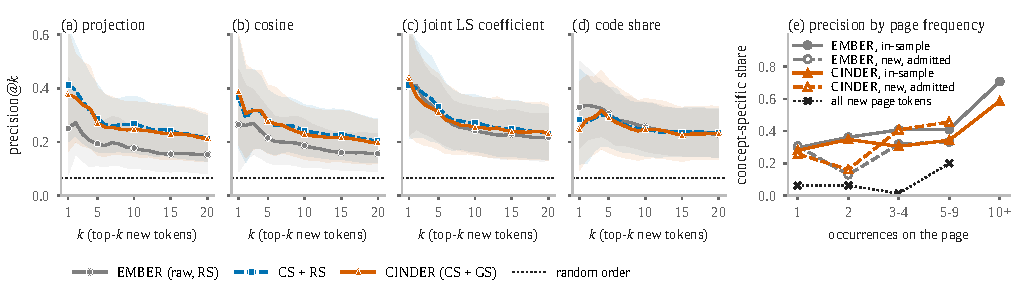
\includegraphics[width=\textwidth]{figures/extrapolation.pdf}
  \caption{Extrapolating a fixed dictionary to concept-only tokens outside the 300 sampled sentences (17 concepts, 5 seeds, balanced condition). (a)--(d)~Precision@$k$: share of the top-$k$ new concept-only tokens by each score that are blindly labelled concept-specific, mean over concepts with 95\% bootstrap bands; dotted: random order (\expnum{0.065}). (e)~Concept-specific share by the token's number of occurrences on the concept's page, for the tokens of the in-sample support (solid) and the new tokens admitted by the 1\% re-solve (dashed); dotted: all new page tokens. Bins with fewer than 5 concepts are omitted.}
  \label{fig:extrapolation}
\end{figure*}
